\documentclass[a4paper, 12pt]{article}

\usepackage{/Users/zhengz/Desktop/Math/Workspace/Homework1/homework}
%%%%%%%%%%%%%%%%%%%%%%%%%%%%%%%%%%%%%%%%%%%%%%%%%%%%%%%%%%%%%%%%%%%%%%%%%%%%%%%%%%%%%%%%%%%%%%%%%%%%%%%%%%%%%%%%%%%%%%%%%%%%%%%%%%%%%%%%
\begin{document}
%Header-Make sure you update this information!!!!
\noindent
%%%%%%%%%%%%%%%%%%%%%%%%%%%%%%%%%%%%%%%%%%%%%%%%%%%%%%%%%%%%%%%%%%%%%%%%%%%%%%%%%%%%%%%%%%%%%%%%%%%%%%%%%%%%%%%%%%%%%%%%%%%%%%%%%%%%%%%%
\large\textbf{Zhengdong Zhang} \hfill \textbf{Homework - Week 7}   \\
Email: zhengz@uoregon.edu \hfill ID: 952091294 \\
\normalsize Course: MATH 634 - Algebraic Topology  \hfill Term: Fall 2024\\
Instructor: Dr.Patricia Hersh \hfill Due Date: $23^{th}$ November, 2024 \\
\noindent\rule{7in}{2.8pt}
\setstretch{1.1}
%%%%%%%%%%%%%%%%%%%%%%%%%%%%%%%%%%%%%%%%%%%%%%%%%%%%%%%%%%%%%%%%%%%%%%%%%%%%%%%%%%%%%%%%%%%%%%%%%%%%%%%%%%%%%%%%%%%%%%%%%%%%%%%%%%%%%%%%
% Exercise 2.2.2
%%%%%%%%%%%%%%%%%%%%%%%%%%%%%%%%%%%%%%%%%%%%%%%%%%%%%%%%%%%%%%%%%%%%%%%%%%%%%%%%%%%%%%%%%%%%%%%%%%%%%%%%%%%%%%%%%%%%%%%%%%%%%%%%%%%%%%%%
\begin{problem}{2.2.2}
Given a map \(f:S^{2n}\rightarrow S^{2n}\), show that there is some point \(x\in S^{2n}\) with either \(f(x)=x\) or \(f(x)=-x\). Deduce that every map 
\(\mathbb{R}P^{2n}\rightarrow \mathbb{R}P^{2n}\) has a fixed point. Construct maps \(\mathbb{R}P^{2n-1}\rightarrow \mathbb{R}P^{2n-1}\) without fixed points from linear 
transformations \(\mathbb{R}^{2n}\rightarrow \mathbb{R}^{2n}\) without eigenvectors.
\end{problem}
\begin{solution}
Assume the opposite. If \(f\) does not have a fix point, then \(f\) is homotopic to the antipodal map \(a\). For every point \(x\in S^{2n}\), we know that \(f(x)\neq a(x)\), so \(f\) is also homotopic to 
\(a\circ a=id\). This implies the antipodal map \(a\) is homotopic to \(id\), but we know 
\[\deg a=(-1)^{2n+1}=-1\neq \deg id.\]
This gives us a contradiction. 

Now given a map \(g:\mathbb{R}\mathbb{P}^{2n}\rightarrow \mathbb{R}\mathbb{P}^{2n}\), Consider the quotient map \(q:S^{2n}\rightarrow \mathbb{R}\mathbb{P}^{2n}\) and the composition:
\[S^{2n}\xrightarrow{q}\mathbb{R}\mathbb{P}^{2n}\xrightarrow{g}\mathbb{R}\mathbb{P}^{2n}.\]
Note that \(q\) is also the universal covering. By Proposition 1.33 in the book, \(g\circ q:S^{2n}\rightarrow \mathbb{R}\mathbb{P}^{2n}\) can be lifted to \(S^{2n}\) if and only if 
\[(g\circ q)_*(\pi_1(S^{2n}))\subseteq q_*(\pi_1(S^{2n})).\]
This can be done because \(S^{2n}\) is simply connected for \(n>0\). So we have a commutative diagram:
\[\begin{tikzcd}
	&& {S^{2n}} \\
	{S^{2n}} & {\mathbb{R}\mathbb{P}^{2n}} & {\mathbb{R}\mathbb{P}^{2n}}
	\arrow["q", from=1-3, to=2-3]
	\arrow["{\bar{g}}", dashed, from=2-1, to=1-3]
	\arrow["q"', from=2-1, to=2-2]
	\arrow["g"', from=2-2, to=2-3]
\end{tikzcd}\]
There exists a point \(x\in S^{2n}\) such that \(\bar{g}(x)=x\) or \(\bar{g}(x)=-x\), and in \(\mathbb{R}\mathbb{P}^{2n}\) we know \(x\) and \(-x\) is identified, so \(g\) has a fixed point.

Consider the linear map \(f:\mathbb{R}^{2n}\rightarrow \mathbb{R}^{2n}\) defined by the following matrix \(A\):
\[\begin{pmatrix}
    0 & 1 &  &  &  &  &  \\
    -1 & 0 &  &  &  &  &  \\
     &  & 0 & 1 &  &  &  \\
     &  & -1 & 0 &  &  &  \\
     &  &  &  & \ddots &  &  \\
     &  &  &  &  & 0 & 1 \\
     &  &  &  &  & -1 & 0 
    \end{pmatrix}\]
\(A\) has no eigenvalue in \(\mathbb{R}\), so it does not have eigenvectors. View every point in \(\mathbb{R}\mathbb{P}^{2n-1}\) as a line through origin in \(\mathbb{R}^{2n}\). The linear map \(f\) defines a map 
\(\bar{f}:\mathbb{R}\mathbb{P}^{2n-1}\rightarrow \mathbb{R}\mathbb{P}^{2n-1}\) has no fixed point because every line in \(\mathbb{R}^{2n}\) is mapped to another line under \(f\) (\(f\) has no eigenvector).
\end{solution}

\noindent\rule{7in}{2.8pt}
%%%%%%%%%%%%%%%%%%%%%%%%%%%%%%%%%%%%%%%%%%%%%%%%%%%%%%%%%%%%%%%%%%%%%%%%%%%%%%%%%%%%%%%%%%%%%%%%%%%%%%%%%%%%%%%%%%%%%%%%%%%%%%%%%%%%%%%%
% Exercise 2.2.4
%%%%%%%%%%%%%%%%%%%%%%%%%%%%%%%%%%%%%%%%%%%%%%%%%%%%%%%%%%%%%%%%%%%%%%%%%%%%%%%%%%%%%%%%%%%%%%%%%%%%%%%%%%%%%%%%%%%%%%%%%%%%%%%%%%%%%%%%
\begin{problem}{2.2.4}
Construct a surjective map \(S^n\rightarrow S^n\) of degree zero, for each \(n\geq 1\).
\end{problem}
\begin{solution}
When \(n=1\), parametrize the unit circle \(S^1\) in complex coordinates \(e^{i t}\) for \(0\leq t\leq 2\pi\) and consider the following map from \(S^1\) to \(S^1\):
\[f_1(e^{i t})=\begin{cases}
    e^{2 i t},&\  0\leq t\leq \pi,\\ 
    e^{-2i(t-\pi)},&\ \pi\leq t\leq 2\pi.
\end{cases}\]
It is obvious that \(f_1\) is continous and surjective. We claim that \(\deg f_1=0\). Indeed, consider the point \(z=-1=e^{i\pi}=e^{-i\pi}\), it has two preimage \(t_1=\frac{\pi}{2}\) and \(t_2=\frac{3\pi}{2}\). 
Choose a neighbourhood \(U_1\) and \(U_2\) around \(t_1\) and \(t_2\) repesctively and let \(U_1\cap U_2=\varnothing \). \(f_1\) on \(U_1\) is a homeomorphism with the same direction but on \(U_2\) is a homeomorphism with 
the reverse direction, so by local degree theorem, \(\deg f_1=\deg f|_{t_1}+\deg f|_{t_2}=1+(-1)=0\). \(f_1:S^1\rightarrow S^1\) is a surjective map of degree zero.

Define \(f_n:S^n\rightarrow S^n\) inductively as \(f_n=Sf_{n-1}\) where \(S\) is the suspension. By Proposition 2.33, we have
\[\deg f_n=\deg f_{n-1}=\cdots=\deg f_1=0.\] 
And for every \(n\), every \(f_n\) is surjective since \(f_1\) is surjective.
\end{solution}

\noindent\rule{7in}{2.8pt}
%%%%%%%%%%%%%%%%%%%%%%%%%%%%%%%%%%%%%%%%%%%%%%%%%%%%%%%%%%%%%%%%%%%%%%%%%%%%%%%%%%%%%%%%%%%%%%%%%%%%%%%%%%%%%%%%%%%%%%%%%%%%%%%%%%%%%%%%
% Exercise 2.2.6
%%%%%%%%%%%%%%%%%%%%%%%%%%%%%%%%%%%%%%%%%%%%%%%%%%%%%%%%%%%%%%%%%%%%%%%%%%%%%%%%%%%%%%%%%%%%%%%%%%%%%%%%%%%%%%%%%%%%%%%%%%%%%%%%%%%%%%%%
\begin{problem}{2.2.6}
Show that every map \(S^n\rightarrow S^n\) can be homotoped to have a fixed point if \(n>0\).
\end{problem}
\begin{solution}
We embed \(S^n\) into \(R^{n+1}\) via the set 
\[S^n=\left\{ (x_0,\ldots,x_n)\in \mathbb{R}^{n+1}\,|\, x_0^2+\cdots+x_n^2=1 \right\}.\]
For \(0\leq i<j\leq n\), let \(R_{ij}\) denote the rotation by degree \(\pi\) of \(S^n\) with respect to the axis normal to the \(x_ix_j\)-plane.

\begin{claim}
Every \(R_{ij}\) is homotopic to the identity map \(id:S^n\rightarrow S^n\).
\end{claim}
\begin{claimproof}
Without loss of generality, assume \(i=0\) and \(j=1\). Write \(r=\sqrt{1-\sum_{k=2}^{n} x_k^2}\). We have a change of variable
\begin{align*}
    x_0& =r\cos (\alpha),\\ 
    x_1& =r\sin (\alpha)
\end{align*}
for \(0\leq \alpha\leq 2\pi\). Consider the following homotopy \(F\):
\begin{align*}
    F:&I\times S^n\rightarrow S^n,\\ 
    &(t,r,\alpha)\mapsto (r,\alpha+t\pi).
\end{align*}
\(F\) is continous and \(F(0,-)=id\), \(F(1,-)\) changes only the coordinates \(x_0,x_1\) and is just a rotation by \(\pi\).
\end{claimproof}

Note that for \((x_0,\ldots,x_n)\in S^n\), we have 
\[R_{ij}(x_0,\ldots,x_n)=(x_0,\ldots,-x_i,\ldots,-x_j,\ldots,x_n).\]
Given a map \(f:S^n\rightarrow S^n\), suppose \(n\) is an even number. If \(f\) has a fixed point, then we are done. If \(f\) does not have a fixed point, then by Exercise 2.2.2, we know that there exists some point 
\(x\in S^n\) such that \(f(x)=-x\). In this case \((R_{n-1,n}\circ \cdots\circ R_{23}\circ R_{01}\circ f)(x)=x\) since \(R_{ij}\) flip the signs of \(x_i,x_j\) and \(n\) is an even number. From the claim, we know that 
for any \(0\leq i<j\leq n\), \(R_{ij}\circ f\) is homotopic to \(id\circ f=f\).

Now assume \(n\) is an odd number. If \(f\) does not have a fixed point, then \(f\) is homotopic to the antipodal map \(a:S^n\rightarrow S^n,\  a(x)=-x\). Consider 
\[S^{n-1}=\left\{ (0,x_1,\ldots,x_n)\in \mathbb{R}^{n+1}\,|\, x_1^2+\cdots+x_n^2=1 \right\}\subseteq S^n.\]
We know that \(a(0,x_1,\ldots,x_n)=(0,-x_1,\ldots,-x_n)\) is still the antipodal map when restricted \(S^{n-1}\), by the previous discussion on even spheres, we know we can \(f\) can be homotoped to have a fixed point.
\end{solution}

\noindent\rule{7in}{2.8pt}
%%%%%%%%%%%%%%%%%%%%%%%%%%%%%%%%%%%%%%%%%%%%%%%%%%%%%%%%%%%%%%%%%%%%%%%%%%%%%%%%%%%%%%%%%%%%%%%%%%%%%%%%%%%%%%%%%%%%%%%%%%%%%%%%%%%%%%%%
% Exercise 2.2.8
%%%%%%%%%%%%%%%%%%%%%%%%%%%%%%%%%%%%%%%%%%%%%%%%%%%%%%%%%%%%%%%%%%%%%%%%%%%%%%%%%%%%%%%%%%%%%%%%%%%%%%%%%%%%%%%%%%%%%%%%%%%%%%%%%%%%%%%%
\begin{problem}{2.2.8}
A polynomial \(f(z)\) with complex coefficients, viewed as a map \(\mathbb{C}\rightarrow \mathbb{C}\), can always be extended to a continous map of one-point compactification 
\(\hat{f}:S^2\rightarrow S^2\). Show that the degree of \(\hat{f}\) equals the degree of \(f\) as a polynomial. Show also that the local degree of \(\hat{f}\) at a root of \(f\) is the 
multiplicity of the root.
\end{problem}
\begin{solution}
Identify \(S^2\) with the complex projective space \(\mathbb{C}\mathbb{P}^1\). \(\mathbb{C}\subset \mathbb{C}\mathbb{P}^1\) has projective coordinates \([z:1]\), and the point \(\infty\in \mathbb{C}\mathbb{P}^1\) has coordinate 
\([0:1]\). Let \(f:\mathbb{C}\rightarrow \mathbb{C}\) be a polynomial \(f(z)=a_nz^n+\cdots+a_1z+a_0\). We can extend \(f\) to a map \(\mathbb{C} \mathbb{P}^1\rightarrow \mathbb{C} \mathbb{P}^1\) by sending \([z:w]\) to \([\sum_{i=0}^{n}a_iz^iw^{n-i}:w^n]\). This map 
is well-defined and continous and if restricted to \(\mathbb{C}\cong \left\{ [z:w]\in \mathbb{C}\mathbb{P}^1\,|\, w=1 \right\}\), this map is just \(f:\mathbb{C}\rightarrow \mathbb{C}\). We call it \(\hat{f}\).  Let \(S\) be the preimage 
of \([0:1]\) under \(\hat{f}\). We have 
\[S=\left\{ [z:1]\in \mathbb{C} \mathbb{P}^1\,|\, z\in \mathbb{C}\ \text{and}\ \hat{f}(z)=0 \right\}.\]
Since \(\mathbb{C}\) is algebraically closed, we can write 
\[f(z)=c(z-z_1)^{i_1}(z-z_2)^{i_2}\cdots(z-z_k)^{i_k}\]
where \(z_1,z_2,\ldots,z_k\in \mathbb{C}\), \(c\in C^*\) and \(i_1,i_2,\ldots,i_k\) are positive integers satisfying \(i_1+\cdots\i_k=n\). 

\begin{claim}
Given a polynomial \(f:\mathbb{C}\rightarrow \mathbb{C}\) where \(f(z)=c(z-a)^n\) for some \(n\geq 2\). The extension \(\hat{f}\) is homotopic to an extension of a polynomial \(g\) which has \(n\) different roots in \(\mathbb{C}\).
\end{claim}
\begin{claimproof}
Without loss of generality, assume \(a=0\). Choose a very small real positive \(\varepsilon>0\) and \(n\) different complex numbers \(a_1,\ldots,a_n\) such that for \(i=1,2,\ldots,n\), we have \(|a_i|<\varepsilon\). Define \(g(z)=\prod_{i=1}^{n}(z-a_i)\) and a map 
\[F:I\times \mathbb{C}\rightarrow \mathbb{C}\, ,\, (t,z)\mapsto tg(z)+(1-t)f(z).\]
This map is obviously continous on \(\mathbb{C}\) and we need to show that it can be extended continouly to \(\mathbb{C}\mathbb{P}^1\). This is the same as showing that the zeros of \(F\) is bounded for \(t\in [0,1]\). This is true because \(f\) and \(g\) have the same degree, so \(\frac{f(z)}{g(z)}\) and 
\(\frac{g(z)}{f(z)}\) is always bounded when \(|z|\to \infty\).
\end{claimproof}

From the above claim, we can assume \(f(z)=\prod_{i=1}^n(z-z_i)\) for different \(z_1,z_2,\ldots,z_n\in \mathbb{C}\). Choose a neighborhood \(U\) of \(z_1\) whcih does not contain \(z_2,\ldots,z_n\). Locally on \(U\), \(f\) can be 
written as \(z\mapsto z-z_1\) is an orientation-preserving homeomorphism (it is just a translation), so \(\deg f|_{z_1}=1\). By the local degree theorem, we have \(\deg f=\sum_{i=1}^n \deg f|_{z_i}=n\), which is equal to the degree of \(f\) as a polynomial.

Now consider a polynomial 
\[f(z)=(z-z_0)^m(z-z_1)\cdots(z-z_n)\] 
where \(z_0,z_1,\ldots,z_n\in \mathbb{C}\) are different complex numbers and \(m\geq 2\) is an integer. From the previous discussion we know that \(\deg \hat{f}=m+n\) and the local degree at \(z_1,\ldots,z_n\) is \(1\). So by local degree theorem 
\[\deg \hat{f}|_{z_0}=\deg \hat{f}-\sum_{k=1}^{n} \deg \hat{f}|_{z_k}=m+n-n=m.\]
\end{solution}

\noindent\rule{7in}{2.8pt}
%%%%%%%%%%%%%%%%%%%%%%%%%%%%%%%%%%%%%%%%%%%%%%%%%%%%%%%%%%%%%%%%%%%%%%%%%%%%%%%%%%%%%%%%%%%%%%%%%%%%%%%%%%%%%%%%%%%%%%%%%%%%%%%%%%%%%%%%
% Exercise 2.2.9
%%%%%%%%%%%%%%%%%%%%%%%%%%%%%%%%%%%%%%%%%%%%%%%%%%%%%%%%%%%%%%%%%%%%%%%%%%%%%%%%%%%%%%%%%%%%%%%%%%%%%%%%%%%%%%%%%%%%%%%%%%%%%%%%%%%%%%%%
\begin{problem}{2.2.9}
Compute the homology groups of the following \(2\)-complexes.
\begin{enumerate}
\item The quotient of \(S^2\) obtained by identifying north and south poles to a point.
\item \(S^1\times (S^1\vee S^1)\).
\item The space obtained from \(D^2\) by first deleting the interiors of two disjoint subdisks in the interiors of \(D^2\) and then identifying all three resulting boundary circles together 
      via homeomorphisms preserving clockwise orientations of these circles.
\item The quotient space of \(S^1\times S^1\) obtained by identifying points in the circle \(S^1\times \left\{ x_0 \right\}\) that differ by \(\frac{2\pi}{m}\) rotation and identifying points in the circle \(\left\{ x_0 \right\}\times S^1\) that 
    differ by \(\frac{2\pi}{n}\) rotation. 
\end{enumerate}
\end{problem}
\begin{solution}
Write each of the following \(2\)-complex as \(X\).
\begin{enumerate}
\item Connect the north and south pole with one meridian and consider the following CW complex structure on \(X\). \(X\) has one \(0\)-cell, one \(1\)-cell and one \(2\)-cell. The \(0\)-cell is the point obtained from identifying the north and south pole. The \(1\)-cell is 
the meridian we choose, and the \(2\)-cell is the \(S^2\) that we are given at first. The boundary map \(d_1=0\) since we only have one \(0\)-cell. To compute the boundary map \(d_2\), we compute the degree of the attaching map \(\partial S^2=S^1\rightarrow S^1=X^1\). Note that this 
maps the half of \(S^1\) in one direction to the whole \(S^1\) and another half in the opposite direction, so the degree is \(0\), which means \(d_2=0\). We have the following cellular chain complex:
\[0\rightarrow \mathbb{Z}\xrightarrow{0}\mathbb{Z}\xrightarrow{0}\mathbb{Z}\rightarrow 0.\]
So we have \(H_n(X)=\mathbb{Z}\) for \(n=0,1,2\) and \(0\) for all else.
\item 
\[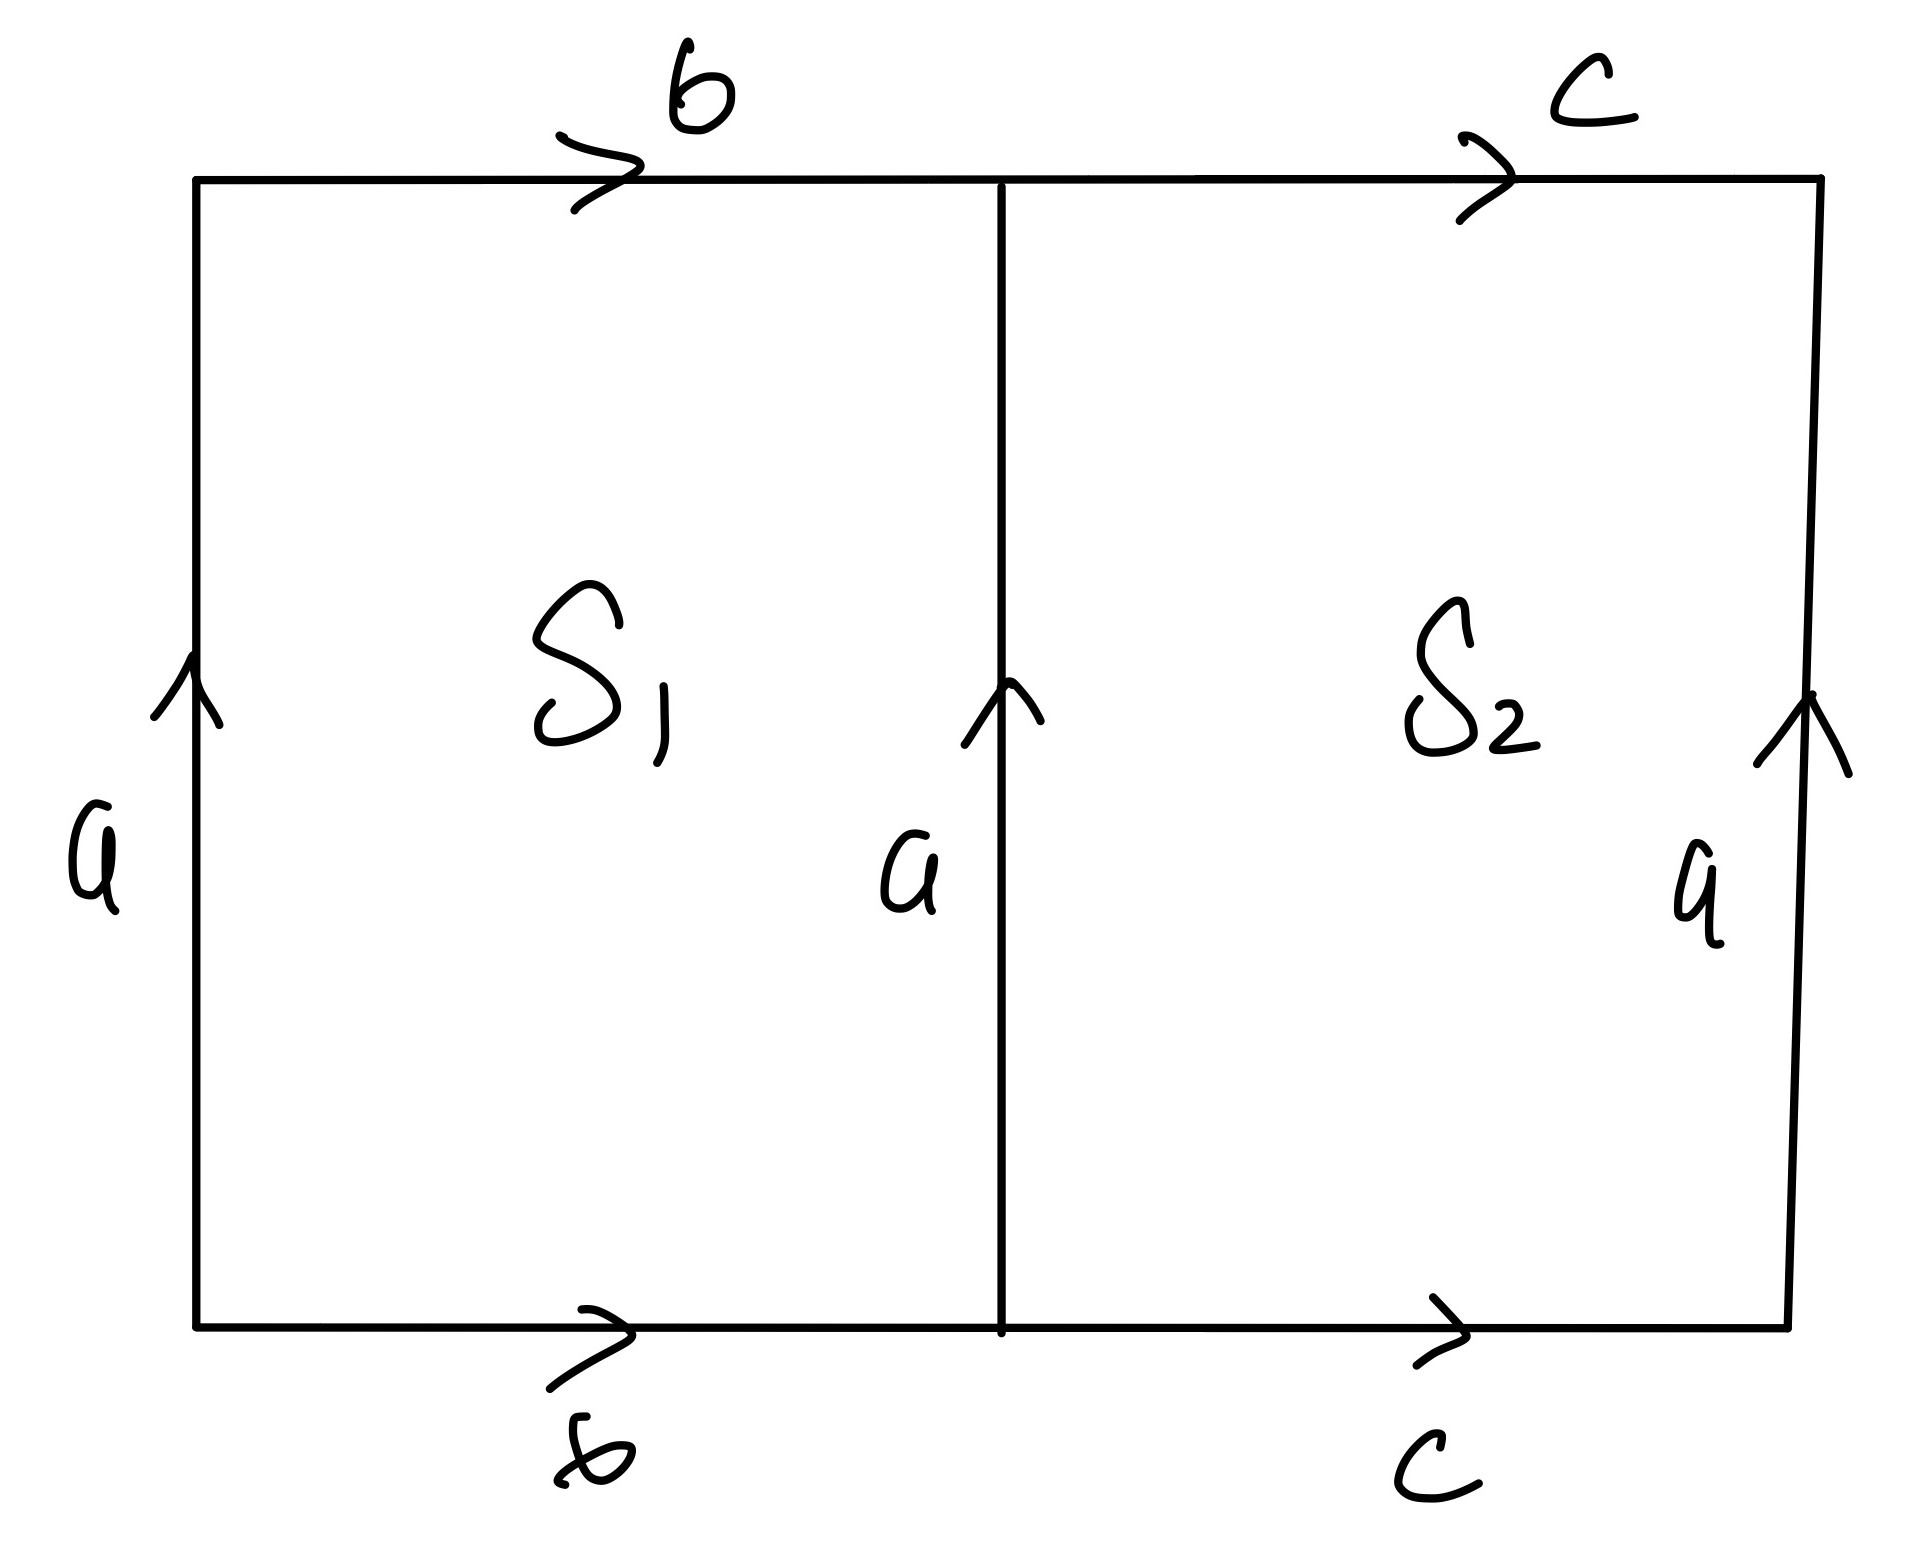
\includegraphics[scale=0.15]{S1timesS1wedgeS1-1.jpg}\]
Consider the CW complex structure of \(X\) above with one \(0\)-cell \(v\), three \(1\)-cell \(a,b,c\) and two \(2\)-cells \(S_1,S_2\). The cellular boundary map \(d_1=0\) since we have one \(0\)-cell. And we can see from the diagram that 
\(d_2(S_1)=a+b-a-b=0\) and \(d_2(S_2)=a+c-a-c\). So we have the following cellular chain complex:
\[0\rightarrow \mathbb{Z}^2\xrightarrow{0}\mathbb{Z}^3\xrightarrow{0}\mathbb{Z}\rightarrow 0.\]
So we have 
\[H_n(X)=\begin{cases}
    \mathbb{Z}\oplus \mathbb{Z}, & n=2,\\ 
    \mathbb{Z}\oplus \mathbb{Z}\oplus \mathbb{Z}, &n=1\\ 
    \mathbb{Z}, &n=0\\ 
    0, & \text{otherwise}.
\end{cases}\]
\item 
\[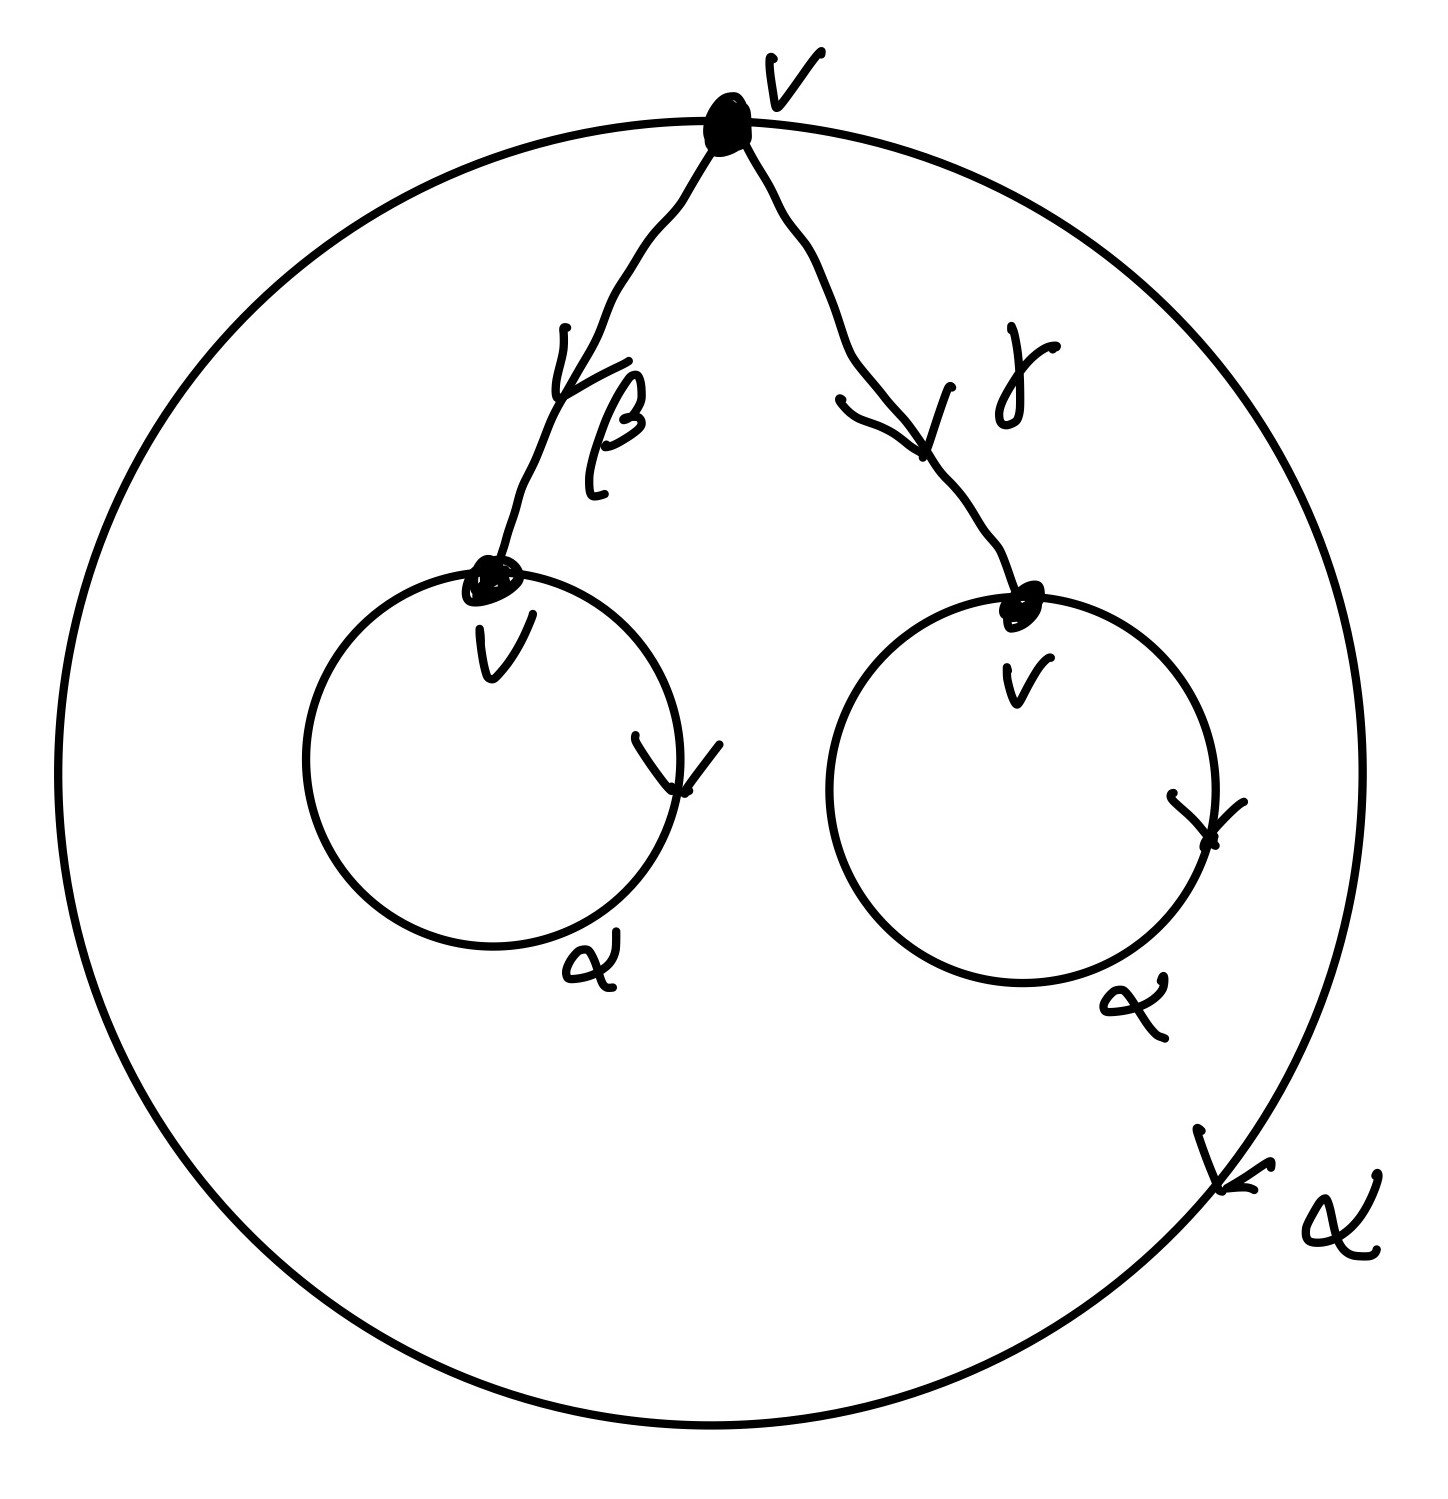
\includegraphics[scale=0.15]{Disk w_o 2d-1.jpg}\]
Consider the CW complex struture of \(X\) given as above. It has one \(0\)-cell \(v\), three \(1\)-cell \(\alpha,\beta,\gamma\) and one \(2\)-cell \(S\). The boundary map \(d_1=0\) since we only have one \(0\)-cell. And 
\[d_2(S)=\alpha+\beta-\alpha-\beta+\gamma-\alpha-\gamma=-\alpha.\]
So We have the following cellular chain complex:
\[0\rightarrow \mathbb{Z}\xrightarrow{d_2}\mathbb{Z}^3\xrightarrow{d_1}\mathbb{Z}\rightarrow 0.\]
We can see that \(\ker d_2=0\) and \(\text{im}\, d_2=\langle -\alpha\rangle\). So \(H_0(X)=\mathbb{Z}\) and 
\[H_1(X)=\langle \alpha,\beta,\gamma\rangle/\langle -\alpha\rangle=\mathbb{Z}\oplus \mathbb{Z}.\]
All other homology groups are zero.
\item Consider the CW complex structure on \(S^1\times S^1\) with one \(0\)-cell, two \(1\)-cell and one \(2\)-cell. The boundary map \(d_1=0\) and \(d_2\) is given by the word \(aba^{-1}b^{-1}\), where \(a\) and \(b\) are \(1\)-cells corresponding to two \(S^1\). Identifying points in \(a\) that differ by \(\frac{2\pi}{m}\) rotation is the same 
as making the attaching map into \(a^m\). So for \(X\), \(d_2\) is given by the word \(a^mb^na^{-m}b^{-n}\). This map is still \(0\) since \(a,a^{-1}\) and \(b,b^{-1}\) appear the same times. So we have a cellular chain complex:
\[0\rightarrow \mathbb{Z}\xrightarrow{0}\mathbb{Z}^2\xrightarrow{0}\mathbb{Z}\rightarrow 0.\]
So we have \(H_n(X)=\mathbb{Z}\) for \(n=0,2\) and \(H_1(X)=\mathbb{Z}\oplus \mathbb{Z}\). All other homology groups are zero.
\end{enumerate}	
\end{solution}

\noindent\rule{7in}{2.8pt}
%%%%%%%%%%%%%%%%%%%%%%%%%%%%%%%%%%%%%%%%%%%%%%%%%%%%%%%%%%%%%%%%%%%%%%%%%%%%%%%%%%%%%%%%%%%%%%%%%%%%%%%%%%%%%%%%%%%%%%%%%%%%%%%%%%%%%%%%
% Exercise 2.2.14
%%%%%%%%%%%%%%%%%%%%%%%%%%%%%%%%%%%%%%%%%%%%%%%%%%%%%%%%%%%%%%%%%%%%%%%%%%%%%%%%%%%%%%%%%%%%%%%%%%%%%%%%%%%%%%%%%%%%%%%%%%%%%%%%%%%%%%%%
\begin{problem}{2.2.14}
A map \(f:S^n\rightarrow S^n\) satisfying \(f(x)=f(-x)\) for all \(x\in S^n\) is called an even map. Show that an even map \(S^n\rightarrow S^n\) must have even degree, and that the degree must in fact be zero when \(n\) is even. When \(n\) is odd, 
show there exist even maps of any given even degree.
\end{problem}
\begin{solution}
Consider the quotient map \(q:S^n\rightarrow \mathbb{R}\mathbb{P}^n\) by identifying \(x\sim -x\). Since \(f(x)=f(-x)\) for all \(x\in S^n\), \(f\) must factor through \(q\):
\[S^n\xrightarrow{q} \mathbb{R}\mathbb{P}^n\xrightarrow{f'}S^n.\]
This induces a map in top homology:
\[H_n(S^n)\xrightarrow{q_*} H_n(\mathbb{R}\mathbb{P}^n)\xrightarrow{f'_*}H_n(S^n).\]
Note that \(q:S^n\rightarrow \mathbb{R}\mathbb{P}^n\) is the two-sheeted covering map. Write \(X=\mathbb{R}\mathbb{P}^n\) and consider the CW complex structure of \(X\) with only one cell in each dimension up to \(n\). Note that 
every \(k\)-skeleton \(X^k\cong \mathbb{R}\mathbb{P}^k\) for \(0\leq k \leq n\). From Example 2.42, we could identify \(H_n(X)=H_n(X^n)\) as the kernel \(d_n:H_n(X^n,X^{n-1})\rightarrow H_{n-1}(X^{n-1},X^{n-2})\). Consider the following diagram:
\[\begin{tikzcd}
	& 0 \\
	{H_n(S^n)} & {H_n(X)} \\
	& {H_n(X^n,X^{n-1})} & {H_{n-1}(X^{n-1},X^{n-2})} \\
	&& {H_{n-1}(X^{n-1})} \\
	&& 0
	\arrow[from=1-2, to=2-2]
	\arrow["{q_*}", from=2-1, to=2-2]
	\arrow["{j_n}"', from=2-2, to=3-2]
	\arrow["{d_n}", from=3-2, to=3-3]
	\arrow["{\partial_n}"', from=3-2, to=4-3]
	\arrow["{j_{n-1}}"', from=4-3, to=3-3]
	\arrow[from=5-3, to=4-3]
\end{tikzcd}\]
We know that \(j_n\circ q_*\) is induced by 
\[S^n\xrightarrow{q}\mathbb{R}\mathbb{P}^n\rightarrow \mathbb{R}\mathbb{P}^n/\mathbb{R}\mathbb{P}^{n-1}\cong S^n.\]
From the Example 2.42, this map has degree \(1+(-1)^n\) and note that \(j_n\) is injective, so \(q_*:H_n(S^n)\cong \mathbb{Z}\rightarrow H_n(\mathbb{R}\mathbb{P}^n)\) is either the zero map if \(n\) is even or 
a map sending \(1\in H_n(S^n)\) to \(2\in H_n(\mathbb{R}\mathbb{P}^n)\cong \mathbb{Z}\) if \(n\) is odd. Therefore, we could conclude that an even map always has even degree, and if \(n\) is even, \(\deg f=0\) since \(H_n(\mathbb{R}\mathbb{P}^n)=0\).

Now assume \(n\) is odd. The Example 2.32 tells us that for every integer \(k\in \mathbb{Z}\), we have a map \(S^1\rightarrow S^1\) of degree \(k\). Since Suspension preserves degree, we have obtained a map \(f_k:S^n\rightarrow S^n\) of degree \(k\). Consider the following 
composition \(f=f_k\circ p\circ q\):
\[S^n\xrightarrow{q}\mathbb{R}\mathbb{P}^n\xrightarrow{p} \mathbb{R}\mathbb{P}^n/\mathbb{R}\mathbb{P}^{n-1}\cong S^n\xrightarrow{f_k}S^n.\]
From the previous discussion, we know that 
\[\deg f=\deg f_k \cdot \deg (p\circ p)=2k.\]
We have constructed a map of degree \(2k\) for every integer \(k\in \mathbb{Z}\).
\end{solution}

\noindent\rule{7in}{2.8pt}
%%%%%%%%%%%%%%%%%%%%%%%%%%%%%%%%%%%%%%%%%%%%%%%%%%%%%%%%%%%%%%%%%%%%%%%%%%%%%%%%%%%%%%%%%%%%%%%%%%%%%%%%%%%%%%%%%%%%%%%%%%%%%%%%%%%%%%%%
% Exercise 2.2.15
%%%%%%%%%%%%%%%%%%%%%%%%%%%%%%%%%%%%%%%%%%%%%%%%%%%%%%%%%%%%%%%%%%%%%%%%%%%%%%%%%%%%%%%%%%%%%%%%%%%%%%%%%%%%%%%%%%%%%%%%%%%%%%%%%%%%%%%%
\begin{problem}{2.2.15}
Show that if \(X\) is a CW compelx then \(H_n(X^n)\) is free by identifying it with the kernel of the cellular boundary map \(H_n(X^n,X^{n-1})\rightarrow H_{n-1}(X^{n-1},X^{n-2})\).	
\end{problem}
\begin{solution}
Consider the following commutative diagram:
\[\begin{tikzcd}
	{H_n(X^{n-1})=0} \\
	& {H_n(X^n)} \\
	&& {H_n(X^n,X^{n-1})} && {H_{n-1}(X^{n-1},X^{n-2})} \\
	&&& {H_{n-1}(X^{n-1})} \\
	&& {H_{n-1}(X^{n-2})=0}
	\arrow[from=1-1, to=2-2]
	\arrow["{j_n}"', from=2-2, to=3-3]
	\arrow["{d_n}", from=3-3, to=3-5]
	\arrow["{\partial_n}"', from=3-3, to=4-4]
	\arrow["{j_{n-1}}"', from=4-4, to=3-5]
	\arrow[from=5-3, to=4-4]
\end{tikzcd}\]
We know by definition \(d_n=j_{n-1}\circ \partial_n\), and from the diagram we can see that \(j_{n-1}\) is injective. So \(\ker d_n=\ker \partial_n\). By exactness, we know that 
\(\ker \partial_n=\text{im} j_n\) and since \(H_n(X^{n-1})=0\), \(j_n\) is injective and we can identify \(H_n(X^n)\) as the kernel of \(d_n\). By Lemma 2.34, \(H_n(X^n,x^{n-1})\) is free abelian, so 
\(H_n(X^n)\cong \ker d_n\) as a subgroup of \(H_n(X^n,X^{n-1})\) is also free.
\end{solution}

\end{document}